%%%%%%%%%%%%%%%%%%%%%%%%%%%%%%%%%%%%%%%%%%%%%%%%%%%%%%%%%%%%%%%%%%%%%%%%
% Plantilla TFG/TFM
% Escuela Politécnica Superior de la Universidad de Alicante
% Realizado por: Jose Manuel Requena Plens
% Contacto: info@jmrplens.com / Telegram:@jmrplens
%%%%%%%%%%%%%%%%%%%%%%%%%%%%%%%%%%%%%%%%%%%%%%%%%%%%%%%%%%%%%%%%%%%%%%%%

\chapter{Antecedentes Metodológicos y Tecnológicos}
\label{Antecedentes Metodológicos y Tecnológicos}
En el siguiente capítulo, se presentan los métodos que son necesarios
conocer para el planteamiento apropiado del método usado para la reconstrucción del cuerpo humano 3D, que constituye el núcleo del presente trabajo.
Primero, se detallará el algoritmo Marching Cubes, que es utilizado más tarde en PIFu que a su vez es el siguiente punto y por último veremos como se van a calcular las comparaciones entre dos modelos 3D diferentes. 

\section{Marching Cubes}
Marching Cubes [\cite{marchingcube}] es un algoritmo utilizado en la reconstrucción del cuerpo humano 3D que es usado en PIFu, este algoritmo genera mallas triangulares de densidad constante desde una función implícita. 

Este algoritmo fue presentado por Lorensen y Cline, calcula los vértices usando un enfoque de divide y vencerás para aproximar la localización en un cubo creado por 8 píxeles, 4 por cada parte del cubo. El algoritmo determina como la superficie intersecta en un cubo y luego se mueve al siguiente cubo (on marchs). Se utiliza una tabla de casos que define la tipología del triángulo.

Este algoritmo tiene 5 fases:
\begin{enumerate}
	\item Determinación del índice caso de cada celda.
	\item Determinación de los bordes intersecados.
	\item Cálculo de intersecciones mediante interpolación lineal.
	\item Triangulación de las intersecciones.
	\item Cálculo de las superficies normales que apuntan hacia fuera.
\end{enumerate}
Marching Cubes procesa cada celda de volumen de forma independiente.[\cite{marchingcubes2}]


\section{PIFu: Pixel-aligned Implicit function}
Como se ha dicho antes en el capítulo \ref{sec:Introducción} PIFu [\cite{pifu}] alinea de manera local las características individuales a nivel de píxel con el contexto global de todo el objeto, esto lo hace de una manera totalmente convolucional y ayuda a no requerir un alto uso de memoria como en otro tipo de representaciones como las que se hacen por vóxel[\cite{bodynet}], esto es importante dado que PIFu es capaz de reconstruir aparte de la forma y pose del cuerpo humano, la ropa, el cabello y los accesorios; por lo tanto la reconstrucción de estos puede ser muy deformable, detallada y con una topología complicada.

\begin{figure}[!h]
	\centering
	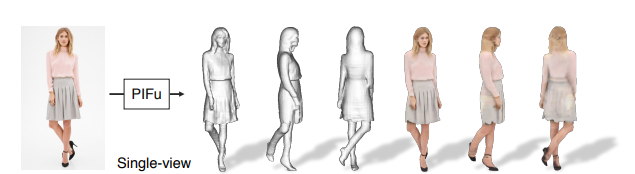
\includegraphics[scale=0.7]{imagenes/antecedentes1.png}
	\caption{Pixel-aligned Implicit function (PIFu) [\cite{pifu}].}
	\label{fig:figura7}
\end{figure}
\pagebreak

Inicialmente se entrena un encoder (codificador) que aprenda sobre vectores de características para cada píxel que existe en la imagen teniendo en cuenta el contexto global relativo a su posición, con este vector y una profundidad en el eje z especificada a lo largo del rayo de cámara saliente del píxel, este aprende a partir de una función implícita que puede clasificar si un punto 3D correspondiente a esta profundidad z está dentro o fuera de la superficie, que en nuestro caso es el cuerpo de una persona.

\subsection{Reconstrucción de la superficie}

Para realizar una buena reconstrucción de manera eficiente en PIFu utiliza una función implícita para definir así la superficie, esta función consiste en un codificador $g$ de imágenes totalmente convolucional y una función $f$ continua e implícita representada por una red MLP (multi-layer perceptrons), donde la superficie esta definida como un conjunto de nivel de:
\begin{equation}
	\label{eq:1}
	f(F(x), z(X)) = s : s \in \mathbb{R}
\end{equation}
Donde para un punto 3D $X$, $x = \pi(X)$ es su proyección 2D, $z(X)$ es el valor de profundidad en el espacio de coordenadas de la cámara, $F(x) = g(I(x))$ es la característica de la imagen en $x$. Se obtiene la función de alineamiento $F(X)$ usando un muestreo bilineal, porque la proyección 2D de $X$ se define en un espacio continuo en lugar de uno discreto (es decir, píxel).
El punto principal de esta función implícita es que aprende a partir del espacio 3D con las características de los píxeles alineados en vez de aprender según las características globales, además esta función se puede presentar como un marco general que puede ser extendido a otras cosas, como por ejemplo predecir los colores RGB.


\begin{figure}[H]
	\centering
	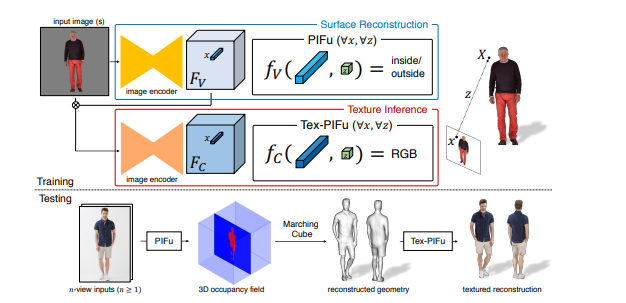
\includegraphics[scale=0.7]{imagenes/antecedentes2.png}
	\caption{Pipeline usada en (PIFu) [\cite{pifu}]. Dada una imagen, PIFu predice la probabilidad continua interior/exterior de un cuerpo humano vestido. Tex-PIFu infiere un valor RGB dados los puntos 3D de la superficie con  con topología arbitraria}
	\label{fig:figura8}
\end{figure}

 Para la reconstrucción de la superficie, se representa como un conjunto de nivel de 0,5 dentro de un campo continuo 3D:
 \begin{equation}
 	\label{eq:2}
 	f_{v}^{*} = \begin{cases}
 				1\text{,}  & \text{X esta dentro de la superficie de la malla}\\
 				0\text{,}  & \text{resto de casos}\\
 			\end{cases}
 \end{equation}

Se entrena la función implícita que alinea píxeles $f_{v}$ minimizando la media del mean squared error (MSE):

\begin{equation}
	\label{eq:3}
	\mathcal{L}_{V} = \frac{1}{n} 
	\sum_{i=1}^{n} | f_{v} (F_{V}(x_{i}) z(X_{i})) - f_{v}^{*}(X_{i}) |^{2}
\end{equation}
 
Donde $X_{i} \in \mathbb{R}^{3}$, $F_{V}(x) = g(I(x))$ es la característica de la imagen del codificador de imágenes $g$ en $x = \pi(X)$ y $n$ es el número de puntos muestrados. Dadas una imagen y la malla 3D correspondiente a la imagen que está espacialmente alineada con la imagen, los parámetros del codificador $g$ y de PIFu $f_{v}$ se actualizan unidas minimizando con la ecuación \ref{eq:3} como [\cite{eq3}] demuestra, el entrenamiento de un codificador de imágenes con un subconjunto de píxeles no le hace daño a la convergencia en comparación a entrenarlo con todos los píxeles[\cite{pifu}]. 

Durante la obtención de la superficie, se muestrea el campo de probabilidad sobre el espacio 3D y se extrae la iso-superficie el campo de probabilidad con un umbral de 0.5 utilizando Marching Cube. 

Este método permite el muestreo directo de puntos 3D sobre la marcha desde la malla en la resolución original utilizando un algoritmo de trazado de rayos eficiente.

\subsection{Obtención de la Textura}
Para la obtención de la textura de la imagen para el modelo 3D, PIFu nos permite predecir de manera directa los colores RGB en la superficie $s$ en la ecuación \ref{eq:4} como un vector con la información de los 3 valores RGB. Sin embargo, extender PIFu a la predicción de colores no es una tarea trivial, ya que los colores están solo definidos en la superficie a diferencia en la reconstrucción tenemos en cuenta todo el espacio 3D. 

Dado unos puntos 3D muestreados en la superficie $X \in \omega$, la función objetivo para la inferencia de textura es el promedio de la función L1 error de los colores como se puede ver en la siguiente ecuación:

\begin{equation}
	\label{eq:4}
	\mathcal{L}_{C} = \frac{1}{n} 
	\sum_{i=1}^{n} | f_{c} (F_{C}(x_{i}) z(X_{i})) - C(X_{i}) |
\end{equation}

Donde $C(X_{i}$ es la verdad básica de los valores de los colores RGB en el punto de superficie $(X_{i} \in \omega$ y $n$ es el numero de puntos muestreados. El problema es que se observó que $f_{c}$ con la función de pérdidas sufría overfitting, esto es provocado porque $f_{c}$ no solo aprende los colores en la superficie sino que también las fronteras de las superficies 3D del objeto por eso $f_{c}$ puede obtener la textura de las  superficies que no se ven con una pose y forma diferente durante la obtención, lo que supone un gran desafío. Para solucionar este problema se realizaron varios cambios, el primero es que la condiciona el codificador de imágenes para la obtención de texturas con las características de la imagen aprendidas en la reconstrucción de la superficie $F_{V}$, con esto el codificador puede enfocarse en la obtención del color dada una geometría incluso los objetos invisibles tienen diferentes formas, poses o topología. Por otro lado se introduce un offset $\epsilon \sim \mathcal{N}(0, d)$ para los puntos de la superficie sobre la superficie normal $N$ así el color puede ser definido no solo por la superficie exacta si no que por el alrededor de este. Con esas modificaciones la función queda así:

\begin{equation}
	\label{eq:5}
	\mathcal{L}_{C} = \frac{1}{n} 
	\sum_{i=1}^{n} | f_{c} (F_{C}(x_{i}^{'}, F{V}), X_{i,z}^{'}) - C(X_{i}) |
\end{equation}

Donde $ X_{i}^{'} = X_{i} + \epsilon$. Se usa un $d = 1.0$ cm para todos los experimentos.

\section{Cálculo de distancias}

Dado que se ha desarrollado

\subsection{Distancia Chamfer}

\subsection{Distancia Hausdorff}


\clearpage
